\documentclass[../main.tex]{subfiles}

\begin{document} %%%%%%%%%%%%%%%%%%%%%%%%%%%%%%%%%%%%%%%%%%%%%%%%%%%%%%%%%%%%
\section{Guía de ejercicios} 
    \subsection{Guía 1}
        \begin{exercise} 
            Una pequeña empresa de productos químicos debe consumir más de 40 $M^3$/mes de un determinado alcohol, debido a que ha firmado un contrato con la municipalidad de la zona (este alcohol es producido allí mismo). En compensación recibe beneficios impositivos. 
            
            Produce dos tipos de fertilizantes: A y B. En la tabla siguiente se da la información básica:
            \begin{table}[ht]
                \centering
                \begin{tabular}{l|l|l|}
                \cline{2-3}
                                                &  \textbf{Producto A} & \textbf{Producto B} \\ \hline
                \multicolumn{1}{|l|}{\textbf{Consumo de alcohol}} & 3 M³/unidad & 2/3 M³/unidad \\ \hline
                \multicolumn{1}{|l|}{\textbf{Consumo de ciclohexano}} & 1 tn/unidad & 2 tn/unidad \\ \hline
                \end{tabular}
                \caption{Tabla de datos}
            \end{table}

            \textbf{Disponibilidad de ciclohexano:} 20 tn. por mes.\\

            Con estas restricciones, y sabiendo que la contribución marginal es 1.200 \$/u para el producto A y 400 \$/u para el producto B, ¿cuál es el plan óptimo de producción?.\\

            \textbf{Solución:}
            \begin{enumerate}
                \item Objetivo del problema: Maximizar la contribución marginal total.
                \item Definir variables de decisión:
                    \begin{equation}
                        \begin{split}
                            x_1 &= \text{unidades producidas de fertilizante A [unidad/mes]} \\
                            x_2 &= \text{unidades producidas de fertilizante B [unidad/mes]} \\
                        \end{split}
                    \end{equation}
                \item Función objetivo (maximizar contribución marginal):
                    \begin{equation}
                        \max Z = 1200 \cdot x_1 + 400 \cdot x_2
                    \end{equation}
                \item Restricciones:
                    \begin{equation}
                        \begin{aligned}
                            3 \cdot x_1 + \frac{2}{3} \cdot x_2 &\geq 40 && \text{(Restricción de consumo de alcohol)} \\
                            x_1 + 2 \cdot x_2 &\leq 20 && \text{(Restricción de consumo de ciclohexano)}\\
                            x_1, x_2 & \geq 0 && \text{(No se pueden producir cantidades negativas de productos)}\\
                        \end{aligned}
                    \end{equation}


            \end{enumerate}

        \end{exercise}

        \begin{exercise}
            Hay tres máquinas disponibles para la producción de dos productos. Cada uno de ellos requiere los tiempos de proceso que se indican en la tabla siguiente (expresados en horas/unidad).
            \begin{table}[ht]
                \centering
                \begin{tabular}{|c|c|c|c|}
                \hline
                \textbf{Producto} & \textbf{Máq. A} & \textbf{Máq. B} & \textbf{Máq. C} \\ \hline
                \textbf{1} &    2      &     3     &    4      \\ \hline
                \textbf{2} &    4      &     2     &    2      \\ \hline
                \textbf{Disponibilidad (hs/mes)} &    80     &    60     &   100     \\ \hline
                \end{tabular}
                \caption{Tabla de datos}
            \end{table}

            El esquema del proceso productivo es el siguiente:
            \begin{itemize}
                \item Ambos productos deben pasar sucesivamente por las tres máquinas (en el orden “A→B→C”) para quedar totalmente terminados. Una máquina puede procesar un solo producto por vez.
                \item El precio de venta de 1 es de 60 \$/u y el de 2 es de 50 \$/u. Se planea la operación para el mes que viene.
            \end{itemize}

            ¿Cuál es el uso óptimo de estos recursos frente al objetivo de maximizar las ganancias?.\\

            \textbf{Solución:}
            \begin{enumerate}
                \item Objetivo del problema: Maximizar las ganancias.
                \item Definir variables:
                    \begin{equation}
                        \begin{split}
                            x_1 &= \text{unidades producidas de producto 1 [unidad/mes]} \\
                            x_2 &= \text{unidades producidas de producto 2 [unidad/mes]} \\
                        \end{split}
                    \end{equation}
                \item Función objetivo (maximizar ganancias):
                    \begin{equation}
                        \max Z = 60 \cdot x_1 + 50 \cdot x_2
                    \end{equation}
                \item Restricciones:
                    \begin{equation}
                        \begin{aligned}
                            2 \cdot x_1 + 4 \cdot x_2 &\leq 80 && \text{(Restricción de disponibilidad de máquina A)} \\
                            3 \cdot x_1 + 2 \cdot x_2 &\leq 60 && \text{(Restricción de disponibilidad de máquina B)}\\
                            4 \cdot x_1 + 2 \cdot x_2 &\leq 100 && \text{(Restricción de disponibilidad de máquina C)}\\
                            x_1, x_2 & \geq 0 && \text{(No se pueden producir cantidades negativas de productos)}\\
                        \end{aligned}
                    \end{equation}
                \item Representación gráfica:
                    \begin{figure}[ht]
                        \centering
                        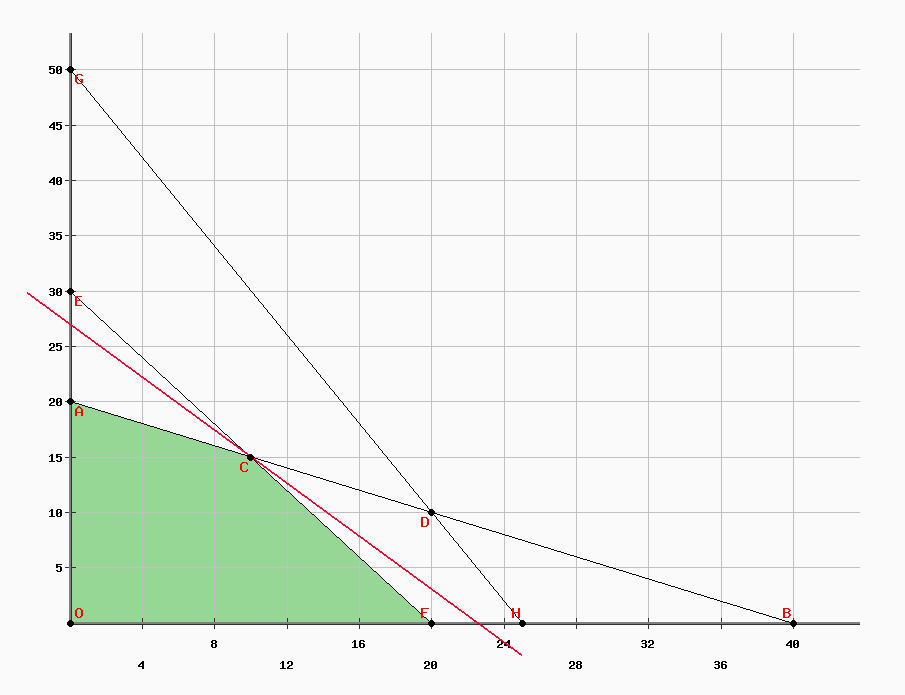
\includegraphics[width=0.9\textwidth]{./images/guia/1-2_ejercicio.png}
                        \caption{Representación gráfica del problema}
                    \end{figure}

                    Observando el gráfico, se puede ver que el punto óptimo es el punto $C(10,15)$, con un valor de $Z = 1350$.

                    \newpage
                    
                \item Obtención algebraicamente de la solución:
                    Tenemos que usar variables de holgura o slack variables para poder expresar las restricciones de igualdad como restricciones de desigualdad. Para ello, definimos las variables de holgura $s_1$, $s_2$ y $s_3$:
                    \begin{equation}
                        \begin{split}
                            s_1 &= \text{variable de holgura de la restricción de disponibilidad de máquina A} \\
                            s_2 &= \text{variable de holgura de la restricción de disponibilidad de máquina B} \\
                            s_3 &= \text{variable de holgura de la restricción de disponibilidad de máquina C} \\
                        \end{split}
                    \end{equation}
                    Con estas variables, podemos expresar las restricciones de igualdad como restricciones de desigualdad:
                    \begin{equation}
                        \begin{aligned}
                            2 \cdot x_1 + 4 \cdot x_2 + s_1 &= 80 && \text{(Restricción de disponibilidad de máquina A)} \\
                            3 \cdot x_1 + 2 \cdot x_2 + s_2 &= 60 && \text{(Restricción de disponibilidad de máquina B)}\\
                            4 \cdot x_1 + 2 \cdot x_2 + s_3 &= 100 && \text{(Restricción de disponibilidad de máquina C)}\\
                            x_1, x_2, s_1, s_2, s_3 & \geq 0 && \text{(No se pueden producir cantidades negativas de productos)}\\
                        \end{aligned}
                    \end{equation}



                    
            \end{enumerate}

        \end{exercise}

        \begin{exercise}
            Se desea definir las cantidades a fabricar de dos productos, A y B cuyo procesamiento se realiza en dos centros de máquinas, conociéndose los datos referentes a los tiempos de proceso y disponibilidades en los centros. Se sabe además que debe cumplirse con un pedido mínimo de 50 unidades de A. Al mismo tiempo, la producción de B debe ser por lo menos cuatro veces superior a la producción de A.
            
            Se conocen los márgenes brutos de beneficio de cada producto.

            \begin{table}[ht]
                \centering
                \begin{tabular}{cc|cc|c|}
                \cline{3-5}
                                                                                                                             &                     & \multicolumn{2}{c|}{\textbf{Producto}}       & \multirow{2}{*}{\textbf{Disponibilidad}} \\ \cline{3-4}
                                                                                                                             &                     & \multicolumn{1}{c|}{\textbf{A}} & \textbf{B} &                                          \\ \hline
                \multicolumn{1}{|c|}{\multirow{2}{*}{\textbf{\begin{tabular}[c]{@{}c@{}}Tiempos\\  unitarios\end{tabular}}}} & \textbf{Máquina I}  & \multicolumn{1}{c|}{1}          & 0,4        & 200                                      \\ \cline{2-5} 
                \multicolumn{1}{|c|}{}                                                                                       & \textbf{Máquina II} & \multicolumn{1}{c|}{0,5}        & 1          & 200                                      \\ \hline
                \multicolumn{2}{|c|}{\textbf{Margen bruto unitario}}                                                                               & \multicolumn{1}{c|}{12}         & 8          &                                          \\ \hline
                \end{tabular}
                \caption{Tabla de datos}
            \end{table}

            \textbf{Solución:}
            \begin{enumerate}
                \item Objetivo del problema: Dado que se quiere maximizar el beneficio, el objetivo es producir la cantidad adecuada de cada producto para maximizar los ingresos.
                \item Definimos variables de decisión:
                    \begin{equation}
                        \begin{split}
                            x_A &= \text{Cantidad de unidades del Producto A a fabricar.} \\
                            x_B &= \text{Cantidad de unidades del Producto B a fabricar.} \\
                        \end{split}
                    \end{equation}
                \item Función objetivo (maximizar beneficio):
                    \begin{equation}
                        \max Z = 12 \cdot x_A + 8 \cdot x_B
                    \end{equation}
                \item Restricciones:
                    \begin{equation}
                        \begin{aligned}
                            x_A &\geq 50 && \text{(Restricción de pedido mínimo de A)} \\
                            x_B &\geq 4 \cdot x_A && \text{(Restricción de producción de B)}\\
                            x_A + 0,4 \cdot x_B &\leq 200 && \text{(Restricción de disponibilidad de máquina I)}\\
                            0,5 \cdot x_A + x_B &\leq 200 && \text{(Restricción de disponibilidad de máquina II)}\\
                            x_A, x_B & \geq 0 && \text{(No se pueden producir cantidades negativas de productos)}\\
                        \end{aligned}
                    \end{equation}
            \end{enumerate}
            
            Nota: 
            
            En este caso $x_A$ y $x_B$ [unidades].

            La Disponibilidad en cada máquina: 200 [unidades].
        \end{exercise}

        \begin{exercise}
            La empresa Seventeen SRL se dedica a la fabricación de manteles de mesa. Fabrica dos modelos que se adaptan al 90\% de las mesas argentinas: el redondo y el rectangular. Cada uno de estos modelos consume 2 y 3 $m^2$ de tela, respectivamente. Además deben ser cortados y cosidos a mano, tarea que lleva una hora para los manteles rectangulares y dos para los redondos (es más complejo el corte). Por último, a los manteles rectangulares se les deben colocar cuatro esquineros de refuerzo.
            
            Semanalmente se pueden conseguir 600 $m^2$ de tela, 600 esquineros y 500 horas de corte y costura. Los márgenes de ganancias son de \$8 para los manteles redondos y \$10 para los rectangulares.\\

            ¿Qué es lo mejor que puede hacer Seventeen con esta información?\\

            \textbf{Solución:}
            \begin{enumerate}
                \item Objetivo del problema: Maximizar el beneficio total.
                \item Definir variables de decisión:
                    \begin{equation}
                        \begin{split}
                            x_C &= \text{Cantidad de manteles redondos (circular) a fabricar.} \\
                            x_R &= \text{Cantidad de manteles rectangulares a fabricar.} \\
                        \end{split}
                    \end{equation}

                    Podemos construir una tabla con los datos de la tabla del enunciado:

                    \begin{table}[ht]
                        \centering
                        \begin{tabular}{c|cc|c|c}
                        \cline{2-4}
                                                                                & \multicolumn{2}{c|}{\textbf{Producto}}                                                                                                               & \multirow{2}{*}{\textbf{Disponibilidad}} &                                        \\ \cline{2-3} \cline{5-5} 
                                                                                & \multicolumn{1}{c|}{\textbf{\begin{tabular}[c]{@{}c@{}}Redondo\\ $x_C$\end{tabular}}} & \textbf{\begin{tabular}[c]{@{}c@{}}Rectangular\\ $x_R$\end{tabular}} &                                          & \multicolumn{1}{c|}{\textbf{Unidades}} \\ \hline
                        \multicolumn{1}{|c|}{\textbf{Consumo de tela}}           & \multicolumn{1}{c|}{2}                                                            & 3                                                                & 600                                      & \multicolumn{1}{c|}{{[}$m^2${]}}          \\ \hline
                        \multicolumn{1}{|c|}{\textbf{Tiempo de corte y costura}} & \multicolumn{1}{c|}{2}                                                            & 1                                                                & 500                                      & \multicolumn{1}{c|}{hs}                \\ \hline
                        \multicolumn{1}{|c|}{\textbf{Esquineros}}                & \multicolumn{1}{c|}{-}                                                            & 4                                                                & 600                                      & \multicolumn{1}{c|}{}                  \\ \hline
                        \multicolumn{1}{|c|}{\textbf{Ganancia}}                  & \multicolumn{1}{c|}{8}                                                            & 10                                                               &                                          & \multicolumn{1}{c|}{\$}                \\ \hline
                        \end{tabular}
                        \caption{Tabla de datos}
                    \end{table}

                \item Función objetivo (maximizar beneficio):
                    \begin{equation}
                        \max Z = 8 \cdot x_C + 10 \cdot x_R
                    \end{equation}
                \item Restricciones:
                    \begin{equation}
                        \begin{aligned}
                            2 \cdot x_C + 3 \cdot x_R &\leq 600 && \text{(Restricción de disponibilidad de tela)} \\
                            2 \cdot x_C + x_R &\leq 500 && \text{(Restricción de disponibilidad de corte y costura)}\\
                            4 \cdot x_R &\leq 600 && \text{(Restricción de disponibilidad de esquineros)}\\
                            x_C, x_R & \geq 0 && \text{(No se pueden producir cantidades negativas de productos)}\\
                        \end{aligned}
                    \end{equation}

            \end{enumerate}
        \end{exercise} 

        \begin{exercise}
            Es necesario alimentar racionalmente un rebaño de cabezas de ganado.

            Los alimentos deben contener imprescindiblemente, cuatro componentes nutritivos: A, B, C y D.

            Se encuentran disponibles en el mercado dos alimentos M y N cuyas propiedades son:
            \begin{itemize}
                \item Un kilogramo de alimento M contiene 100 gr. de nutriente A, 100 gr. de C, y 200 gr. de D.
                \item Un kilogramo de alimento N contiene 100 gr. de nutriente B, 200 gr. de C y 100 gr. de D.
            \end{itemize}

            Cada animal debe consumir como mínimo, por día, 400 gr. de nutriente A, 600 gr. de B, 2.000 gr. de C y 1.700 gr. de D.

            El alimento M cuesta 10 \$/kg, y el N cuesta 4 \$/kg.

            ¿Qué cantidad de alimentos M y N debe suministrarse a cada animal diariamente para que la ración sea la más económica?.\\

            \textbf{Solución:}
            \begin{enumerate}
                \item Objetivo del problema: Minimizar el costo total de la ración.
                \item Definir variables de decisión:
                    \begin{equation}
                        \begin{split}
                            x_M &= \text{Cantidad de alimento M a suministrar [kg/día]} \\
                            x_N &= \text{Cantidad de alimento N a suministrar [kg/día]} \\
                        \end{split}
                    \end{equation}

                    Podemos construir una tabla con los datos de la tabla del enunciado:                    
                    \begin{table}[ht]
                        \centering
                        \begin{tabular}{c|cc|c|}
                        \cline{2-4}
                                                                  & \multicolumn{2}{c|}{\textbf{Producto}}       & \multirow{2}{*}{\textbf{\begin{tabular}[c]{@{}c@{}}Consumo \\ mínimo\end{tabular}}} \\ \cline{1-3}
                        \multicolumn{1}{|c|}{\textbf{Nutrientes}} & \multicolumn{1}{c|}{\textbf{M}} & \textbf{N} &                                                                                     \\ \hline
                        \multicolumn{1}{|c|}{\textbf{A}}          & \multicolumn{1}{c|}{100}        & -          & 400                                                                                 \\ \hline
                        \multicolumn{1}{|c|}{\textbf{B}}          & \multicolumn{1}{c|}{-}          & 100        & 600                                                                                 \\ \hline
                        \multicolumn{1}{|c|}{\textbf{C}}          & \multicolumn{1}{c|}{100}        & 200        & 2000                                                                                \\ \hline
                        \multicolumn{1}{|c|}{\textbf{D}}          & \multicolumn{1}{c|}{200}        & 100        & 1700                                                                                \\ \hline
                        \multicolumn{1}{|c|}{\textbf{Ganancia}}   & \multicolumn{1}{c|}{10}         & 4          &                                                                                     \\ \hline
                        \end{tabular}
                        \caption{Tabla de datos}
                    \end{table}
                    
                \item Función objetivo (minimizar costo total):
                    \begin{equation}
                        \min Z = 10 \cdot x_M + 4 \cdot x_N
                    \end{equation}
                \item Restricciones:
                    \begin{equation}
                        \begin{aligned}
                            100 \cdot x_M &\geq 400 && \text{(Restricción de consumo mínimo de nutriente A)} \\
                            100 \cdot x_N &\geq 600 && \text{(Restricción de consumo mínimo de nutriente B)}\\
                            100 \cdot x_M + 200 \cdot x_N &\geq 2000 && \text{(Restricción de consumo mínimo de nutriente C)}\\
                            200 \cdot x_M + 100 \cdot x_N &\geq 1700 && \text{(Restricción de consumo mínimo de nutriente D)}\\
                            x_M, x_N & \geq 0 && \text{(No se pueden producir cantidades negativas de productos)}\\
                        \end{aligned}
                    \end{equation}
                
            \end{enumerate}
        \end{exercise}

        \begin{exercise} % 1.7
            Dado el siguiente sistema de inecuaciones:
            \begin{equation}
                \begin{aligned}
                    4 \cdot x_1 - 2 \cdot x_2 &\leq 4 \\
                    4 \cdot x_1 + 2 \cdot x_2 &\leq 8 \\
                    x_1 + x_2 &\geq 0 \\
                \end{aligned}
            \end{equation}

            Y el funcional:
            \begin{equation}
                \max Z = 8 \cdot x_1 + 4 \cdot x_2 
            \end{equation}

            \underline{Se pide:}
            \begin{enumerate}[label=\alph*)]
                \item Encontrar un enunciado compatible con el mismo.
                \item Resolverlo gráficamente.
                \item Indicar la o las soluciones del problema que optimicen el funcional.
                \item Dar el valor de las variables débiles o slacks, sus unidades y significado en cada uno de los vértices del poliedro.
            \end{enumerate}

            \textbf{Solución:}
            \begin{enumerate}[label=\alph*)]
                \item
                \item Simulado con la página \cite{PL_online}.
                    %Cargamos imagen
                    \begin{figure}[ht]
                        \centering
                        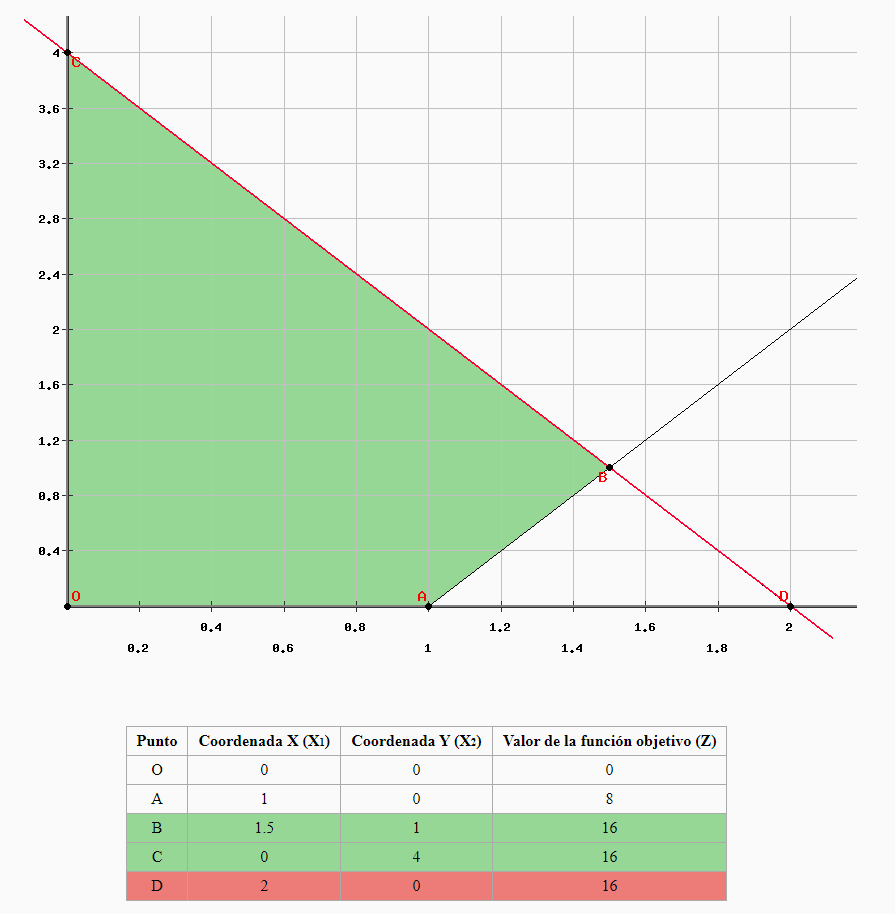
\includegraphics[width=0.8\textwidth]{./images/guia/1-6_ejercicio.png}
                        \caption{Representación gráfica del problema}
                        \label{fig:1-6_ejercicio}
                    \end{figure}
                    
                \item Observando la Figura \ref{fig:1-6_ejercicio}, se puede ver que el punto óptimo es el punto $B(1.5,1)$ y $C(0,4)$, con un valor de $Z = 16$.
            \end{enumerate}
        \end{exercise}

        \newpage

    \subsection{Guía 2}
        \addtocounter{exercise}{-6}
        \setcounter{section}{2} % Reinicia el contador de subsección para la Guía 2

        \begin{exercise} % 2.1
            Un taller de tejido elabora varios modelos de pullóver. Estos modelos de pullóver se pueden agrupar, desde un punto de vista técnico-económico, en tres tipos diferentes de prendas, a los cuales llamaremos A, B y C.

            El taller posee dos máquinas (I y II). Los pullóveres A sólo pueden hacerse en la máquina I, los C sólo pueden hacerse en la máquina II y los B pueden hacerse tanto en la máquina I como en la II.

            Las dos máquinas trabajan dos turnos por día, 8 horas en cada turno, de lunes a viernes.

            La materia prima utilizada es lana de dos calidades distintas (Mejorada y Normal). La lana Mejorada se utiliza para los pullóveres de tipo A y C. Los pullóveres de tipo B se hacen con lana Normal. De la lana Mejorada se pueden conseguir hasta 20 kg./semana y de la lana Normal hasta 36 kg./semana.

            Existe un compromiso de entregar 10 pullóveres B por semana a un importante distribuidor.

            No es necesario que las prendas que comienzan a fabricarse en una semana se terminen durante la misma, es decir que pueden quedar pullóveres a medio hacer de una semana para la próxima.

            Los estándares de producción y materia prima y los beneficios unitarios para cada tipo de pullóver, se indican en el siguiente cuadro:
            
            ¿Qué es lo mejor que se puede hacer con la información disponible?

            \begin{table}[ht]
                \centering
                \begin{tabular}{|c|cc|cc|c|}
                \hline
                \multirow{3}{*}{\textbf{\begin{tabular}[c]{@{}c@{}}Tipo de\\ pullóver\end{tabular}}} & \multicolumn{2}{c|}{\textbf{\begin{tabular}[c]{@{}c@{}}Estándar de producción\\ hs/pullover\end{tabular}}} & \multicolumn{2}{c|}{\textbf{\begin{tabular}[c]{@{}c@{}}Estándar de materia prima\\ kg/pullover\end{tabular}}} & \multirow{3}{*}{\textbf{\begin{tabular}[c]{@{}c@{}}Beneficio \\ unitario \\ \$/pullover\end{tabular}}} \\ \cline{2-5}
                                                                                                     & \multicolumn{1}{c|}{\multirow{2}{*}{\textbf{Máquina I}}}       & \multirow{2}{*}{\textbf{Máquina II}}      & \multicolumn{1}{c|}{\multirow{2}{*}{\textbf{Mejorada}}}           & \multirow{2}{*}{\textbf{Normal}}          &                                                                                                        \\
                                                                                                     & \multicolumn{1}{c|}{}                                          &                                           & \multicolumn{1}{c|}{}                                             &                                           &                                                                                                        \\ \hline
                \textbf{A}                                                                           & \multicolumn{1}{c|}{5}                                         & -                                         & \multicolumn{1}{c|}{1,6}                                          & -                                         & 10                                                                                                     \\ \hline
                \textbf{B}                                                                           & \multicolumn{1}{c|}{6}                                         & 4                                         & \multicolumn{1}{c|}{-}                                            & 1,8                                       & 15                                                                                                     \\ \hline
                \textbf{C}                                                                           & \multicolumn{1}{c|}{-}                                         & 4                                         & \multicolumn{1}{c|}{1,2}                                          & -                                         & 18                                                                                                     \\ \hline
                \end{tabular}
                \caption{Tabla de datos}
            \end{table}

            \textbf{Solución:}
            \begin{enumerate}
                \item Objetivo del problema: Maximizar el beneficio total.
                \item Variables de decisión:
                    \begin{equation}
                        \begin{split}
                            x_A &= \text{Cantidad de pullóveres A a fabricar.} [pullover/semana] \\
                            x_B &= \text{Cantidad de pullóveres B a fabricar.} [pullover/semana] \\
                            x_C &= \text{Cantidad de pullóveres C a fabricar.} [pullover/semana]\\
                        \end{split}
                    \end{equation}
                \item Función objetivo (maximizar beneficio):
                    \begin{equation}
                        \max Z = 10 \cdot x_A + 15 \cdot x_B + 18 \cdot x_C
                    \end{equation}
                \item Restricciones:
                    \begin{itemize}
                        \item Restricción de disponibilidad de máquina I:
                            \begin{equation}
                                \begin{aligned}
                                    5 \frac{hs}{pullover} \cdot x_A + 6 \frac{hs}{pullover} \cdot x_B &\leq 2 \frac{turno}{dia} \cdot 8 \frac{hs}{turno} \cdot 5 \frac{dia}{semana} \\
                                    5 \frac{hs}{pullover} \cdot x_A + 6 \frac{hs}{pullover} \cdot x_B &\leq 80 \frac{hs}{semana} \\
                                \end{aligned}
                            \end{equation}
                        \item Restricción de disponibilidad de lana Mejorada:
                            \begin{equation}
                                \begin{aligned}
                                    1,6 \frac{kg}{pullover} \cdot x_A + 1,2 \frac{kg}{pullover} \cdot x_C &\leq 20 \frac{kg}{semana} \\
                                \end{aligned}
                            \end{equation}
                    \end{itemize}

                    Todas las restrcciones son:
                    \begin{equation}
                        \begin{aligned}
                            5 \cdot x_A + 6 \cdot x_B &\leq 80 && \text{(Restricción de disponibilidad de máquina I)} \\
                            4 \cdot x_B + 4 \cdot x_C &\leq 80 && \text{(Restricción de disponibilidad de máquina II)}\\
                            1,6 \cdot x_A + 1,2 \cdot x_C &\leq 20 && \text{(Restricción de disponibilidad de lana Mejorada)}\\
                            1,8 \cdot x_B &\leq 36 && \text{(Restricción de disponibilidad de lana Normal)}\\
                            x_B &\geq 10 && \text{(Restricción de compromiso de entrega de pullóveres B)}\\
                            x_A, x_B, x_C & \geq 0 && \text{(No se pueden producir cantidades negativas de productos)}\\
                        \end{aligned}
                    \end{equation}
            \end{enumerate}


        \end{exercise}

        \begin{exercise} % 2.2
            “Copani”, una compañía dedicada a la minería, explota tres yacimientos (Sierra Alta, Sierra Chica y El Abra), de cada uno de los cuales obtiene un mineral que contiene cuatro metales: Cobre, Estaño, Manganeso y Zinc. Con estos cuatro metales, y siguiendo las especificaciones que pueden verse en el cuadro que figura a continuación, Copani elabora dos aleaciones: A y B.

            \begin{table}[h]
                \centering
                \begin{tabular}{|c|c|}
                \hline
                Aleación           & Especificaciones              \\ \hline
                \multirow{3}{*}{A} & Como máximo 80\% de Cobre     \\ \cline{2-2} 
                                   & Como máximo 30\% de Estaño    \\ \cline{2-2} 
                                   & Como mínimo 50\% de Zinc      \\ \hline
                \multirow{3}{*}{B} & Entre 40\% y 60\% de Estaño   \\ \cline{2-2} 
                                   & Como mínimo 30\% de Manganeso \\ \cline{2-2} 
                                   & Como máximo 70\% de Zinc      \\ \hline
                \end{tabular}
                \caption{Especificaciones de las aleaciones}
            \end{table} 
            
            \newpage

            La proporción de cada metal que está en el mineral depende del yacimiento del cual proviene ese mineral. La siguiente tabla indica esos datos, así como los costos de extracción de mineral:

            \begin{table}[h]
                \centering
                \begin{tabular}{|c|c|ccccc|c|}
                \hline
                \multirow{3}{*}{\textbf{Mineral}} & \multirow{3}{*}{\textbf{\begin{tabular}[c]{@{}c@{}}Máximo \\ Disponible \\ (toneladas)\end{tabular}}} & \multicolumn{5}{c|}{\multirow{2}{*}{\textbf{Porcentaje de Metal}}}                                                                                                         & \multirow{3}{*}{\textbf{\begin{tabular}[c]{@{}c@{}}Costo \\ \$/Tonelada\end{tabular}}} \\
                                                  &                                                                                                       & \multicolumn{5}{c|}{}                                                                                                                                                      &                                                                                        \\ \cline{3-7}
                                                  &                                                                                                       & \multicolumn{1}{c|}{\textbf{Cobre}} & \multicolumn{1}{c|}{\textbf{Estaño}} & \multicolumn{1}{c|}{\textbf{Manganeso}} & \multicolumn{1}{c|}{\textbf{Zinc}} & \textbf{Otros} &                                                                                        \\ \hline
                \textbf{Sierra Alta}              & 1000                                                                                                  & \multicolumn{1}{c|}{20}             & \multicolumn{1}{c|}{10}              & \multicolumn{1}{c|}{30}                 & \multicolumn{1}{c|}{30}            & 10             & 10                                                                                     \\ \hline
                \textbf{Sierra Chica}             & 2000                                                                                                  & \multicolumn{1}{c|}{10}             & \multicolumn{1}{c|}{20}              & \multicolumn{1}{c|}{30}                 & \multicolumn{1}{c|}{30}            & 10             & 40                                                                                     \\ \hline
                \textbf{El Abra}                  & 3000                                                                                                  & \multicolumn{1}{c|}{5}              & \multicolumn{1}{c|}{5}               & \multicolumn{1}{c|}{70}                 & \multicolumn{1}{c|}{30}            & 0              & 50                                                                                     \\ \hline
                \end{tabular}
                \caption{Tabla de datos}
            \end{table}
            
            La aleación A se vende a \$A por tonelada y la aleación B a \$B por tonelada. Con la información indicada: ¿Qué es lo mejor que puede hacer “Copani”?\\
            
            Para facilitar el análisis se incluyen las siguientes definiciones:
            \begin{itemize}
                \item Aleación: Producto homogéneo de propiedades metálicas, compuesto de dos o más elementos, uno de los cuales, al menos, debe ser un metal. Ej: Bronce, Acero.
                \item Metal: Cada uno de los elementos químicos, buenos conductores del calor y de la electricidad. Ej: Oro, Cobre, Hierro.
                \item Mineral: Sustancia inorgánica que se halla en la superficie o en diversas capas de la tierra, cuya explotación ofrece interés. Ej: Ferrita, Pirita
            \end{itemize}

            \textbf{Solución:}
            \begin{enumerate}
                \item Objetivo del problema: Maximizar el beneficio total reduciendo los costos de extracción de mineral.
                \item Definimos variables de decisión:
                    \begin{equation}
                        \begin{split}
                            y_A &= \text{Cantidad de aleación A producida.} [toneladas] \\
                            y_B &= \text{Cantidad de aleación B producida.} [toneladas] \\\\
                            x_{SA} &= \text{Cantidad de mineral extraído de Sierra Alta.} [toneladas] \\
                            x_{SC} &= \text{Cantidad de mineral extraído de Sierra Chica.} [toneladas] \\
                            x_{EA} &= \text{Cantidad de mineral extraído de El Abra.} [toneladas] \\\\
                        \end{split}
                    \end{equation}

                    Queremos:
                    \begin{equation*}
                        \text{Maximizar Beneficio Total} = \text{Maximizar Ingresos} - \text{Minimizar Costos}
                    \end{equation*}

                    Donde:
                    \begin{equation*}
                        \begin{split}
                            \text{Ingresos} &= \$A \cdot y_A + \$B \cdot y_B \\
                            \text{Costos} &= \$10 \cdot x_{SA} + \$40 \cdot x_{SC} + \$50 \cdot x_{EA} \\
                        \end{split}
                    \end{equation*}
                \item Función objetivo:
                    \begin{equation}
                        \max Z =  A \cdot y_A + B \cdot y_B - (10 \cdot x_{SA} + 40 \cdot x_{SC} + 50 \cdot x_{EA})
                    \end{equation}

                \item Restricciones:
                
                    Las restricciones incluirían la disponibilidad máxima de minerales en cada yacimiento, así como las especificaciones para las aleaciones (porcentajes máximos y mínimos de cada metal)
                    \begin{itemize}
                        \item Restricciones de Cobre, Estaño, Manganeso y Zinc para la aleación A:
                            \begin{equation}
                                \begin{aligned}
                                    0,2 \cdot x_{SA} + 0,1 \cdot x_{SC} + 0,05 \cdot x_{EA} &\leq 0,8 \cdot y_A && \text{(Restricción de Cobre)} \\
                                    0,1 \cdot x_{SA} + 0,2 \cdot x_{SC} + 0,05 \cdot x_{EA} &\leq 0,3 \cdot y_A && \text{(Restricción de Estaño)}\\
                                    0,3 \cdot x_{SA} + 0,3 \cdot x_{SC} + 0,2 \cdot x_{EA} &\geq 0,5 \cdot y_A && \text{(Restricción de Zinc)}\\
                                \end{aligned}
                            \end{equation}
                        \item Restricciones de Estaño, Manganeso y Zinc para la aleación B:
                            \begin{equation}
                                \begin{aligned}
                                    0,4 \cdot y_B \leq 0,1 \cdot x_{SA} + 0,2 \cdot x_{SC} + 0,05 \cdot x_{EA} &\leq 0,6 \cdot y_B && \text{(Restricción de Estaño)}\\
                                    0,3 \cdot x_{SA} + 0,3 \cdot x_{SC} + 0,7 \cdot x_{EA} &\geq 0,3 \cdot y_B && \text{(Restricción de Manganeso)}\\
                                    0,3 \cdot x_{SA} + 0,3 \cdot x_{SC} + 0,3 \cdot x_{EA} &\leq 0,7 \cdot y_B && \text{(Restricción de Zinc)}\\
                                \end{aligned}
                            \end{equation}
                        \item Restricciones de disponibilidad de minerales:
                            \begin{equation}
                                \begin{aligned}
                                    x_{SA} &\leq 1000 && \text{(Restricción de disponibilidad de Sierra Alta)} \\
                                    x_{SC} &\leq 2000 && \text{(Restricción de disponibilidad de Sierra Chica)}\\
                                    x_{EA} &\leq 3000 && \text{(Restricción de disponibilidad de El Abra)}\\
                                \end{aligned}
                            \end{equation}
                        \item Restricciones de no negatividad:
                            \begin{equation}
                                \begin{aligned}
                                    x_{SA}, x_{SC}, x_{EA}, y_A, y_B &\geq 0 && \text{(No se pueden producir cantidades negativas de productos)}\\
                                \end{aligned}
                            \end{equation}
                    \end{itemize}
                    
                \item 
            \end{enumerate}
        \end{exercise}



















\end{document}  %%%%%%%%%%%%%%%%%%%%%%%%%%%%%%%%%%%%%%%%%%%%%%%%%%%%%%%%%%%%%
